\chapter{Related work}
\label{chapter2}

\section{State of the Art}

For mobile systems there are only two main platforms: Android and iOS. Since Android is an open source project, a vast number of smartphone manufacturing companies provide this base operating system and some have even implemented their own wrapper around it. As a result, the device suite for Android has surpassed 7000 devices \cite{Android-Devices}. On the other hand, the iOS platform is much more restrictive and only Apple is allowed to manufacture devices with iOS, which results in the testing advantage of having a smaller device suite \cite{Apple-Devices}. However, due to the secrecy and restrictions of the iOS system (as opposed to Android), there are fewer tools available that may perform automated tests, making test automation fairly more uncommon on this platform. Consequently, quality control might be performed through manual testing instead of automated testing, even if it is not the proper approach.

There are currently a few tools that allow the development of automated user interface tests for iOS. The feasibility of developing tests through one or the other varies depending on the compatibility of the tool with the characteristics of the project. This refers to factors such as: project budget, programming languages with which the team to perform the automation is familiar with, whether the application is hybrid or native, testing load and speed requirements, among many others.

The two types of tools used to create user interface automated tests are: automation APIs/frameworks and record and replay tools \cite{Linares-Vasquez2017ContinuousTesting}. Both types are within the scope of this project. It is also worth noting that there are several other test support tools like: bug and error reporting/monitoring tools, device streaming tools and automated test input generation tools. It is important to understand at a high level how these two tool types work and how they are used to create automated tests.

They both attempt to provide an interface for the user to create automated tests. Which is why, in some cases, test automation frameworks provide both types. Even though the goal is the same, the way the actual automated test is created is where they differ. On the one hand, automation APIs/frameworks require a manually written test script which contains all of the code that makes up the automated test. On the other hand, record and replay tools only require for the test to be manually executed and the tool itself will record all the interactions that where performed, automatically generating the automated test.

During the execution of an automated test, the tool must be capable of interacting with the smartphone GUI elements as a real user would, replicating the test case scenarios. This includes performing GUI interactions such as: swiping, tapping, dragging, pinching, among others.


\section{Test Automation Tools}

There are several different tools that can be used to develop automated tests, ranging from paid license all-in-one tools like Ranorex \cite{Ranorex} to open source client-server tools like Appium \cite{Appium}. 

Getting to know all of the available tools, how they work and how they are used can become a very time-consuming task. Besides, when performing research about test automation tools for iOS, you generally find a small list of tools with a brief description. It turns out, the actual information you can find on automation tools for iOS is very limited and as a result you can easily have a hard time trying to choose the appropriate tool for your project. As a consequence, this project pursues to reduce the conceptual gap present when trying to select the most appropriate user interface test automation tool that supports iOS applications.

Here, a list and a brief description with the most relevant and currently available tools that perform user interface test automation over the iOS platform is shown. This will provide a high level view on what is available and may help you discard some options right away.

\subsection {XCUITest}
Xcode comes with the testing framework XCTest. This testing framework will not only allow you to code your unit tests, but you may also record and write UI tests. This testing tool has seen mayor upgrades since it was released a few years ago and has now become a really solid option. \cite{XCUITest}

\subsection {Appium}
Appium has now become one of the most popular mobile test automation tools out there. This open source project is characterized by a client server architecture which supports a wide range of programming languages and testing frameworks to work on. \cite{Appium}

\subsection {Calabash}
Although Xamarin (Microsoft) discontinued their development for this test automation framework up until iOS 11 and Android 8, it has still been maintained by its community. It works with Cucumber in order to follow the BDD process plus it is a free and open source project. This means it can become fairly simple to write automated tests without much coding experience. \cite{Calabash}

\subsection {EarlGrey (2.0)}
This open source project by Google provides a testing framework works along with the existing XCUITest in order to provide certain advantages such as synchronization and white box testing. \cite{EarlGrey}
	
\subsection {Ranorex}
This paid all-in-one solution seems to be one of the most popular of its kind. It allows the recording and writing of automated tests for many platforms and it is simple to use, for which its users do not need to be skilled with programming to use it. \cite{Ranorex}

\subsection {KIF}
KIF, standing for “Keep It Functional” is a test automation framework that works at the XCTest level and runs with your unit tests. Tests are written in Objective-C and rely on the accessibility attributes. \cite{KIF}

\subsection {Detox}
Detox is a grey-box end to end testing framework for mobile devices (iOS and Android) which provides fast tests with improved reliability regarding flakiness. It is designed to support both React Native and pure native ones and it may perform testing over a real device or a simulator. \cite{Detox}

\subsection {TestComplete}
This paid all-in-one solution provides everything you may need in order to build and run your tests ranging from the testing framework to the physical/virtual devices. You can either write your own tests on any of the 7 available languages or use the built-in record and replay tool. \cite{TestComplete}

\subsection {MonkeyTalk}
MonkeyTalk is a record and replay open source mobile app automation tool. It is designed to be simple to setup and use.   It provides support for both android and iOS. \cite{MonkeyTalk}

\subsection {Quantum}
The Quantum framework allows you to build BDD automated tests using Cucumber. It supports both iOS and Android. Tests are written in Java. \cite{Quantum}

\section{Classification}
Conveniently, it is possible to classify these tools in groups from a high-level standpoint:

1. First-party: Here we have the well known XCTestUI which is easy to setup, reliable to use and requires a moderate amount of experience to work with. The main downside is it does not provide any compatibility with other mobile operating systems like Android.

2. XCTest based: These act as libraries that provide some extra features besides what XCTestUI has to offer. Tools in this group include EarlGrey and KIF.

3. Third Party: Third party tools like Appium, will require the most experience to work on but provide great flexibility and interoperability.

4. All-in-one paid:  These are usually the easiest to use but generally require a paid license. Tools in this group include TestComplete and Ranorex.

\section{Comparison Table}

In the following table, you will be able to visualize a comparison between the main characteristics of the previously mentioned tools. Further on, the case study will provide even more specific information about a few of these tools.

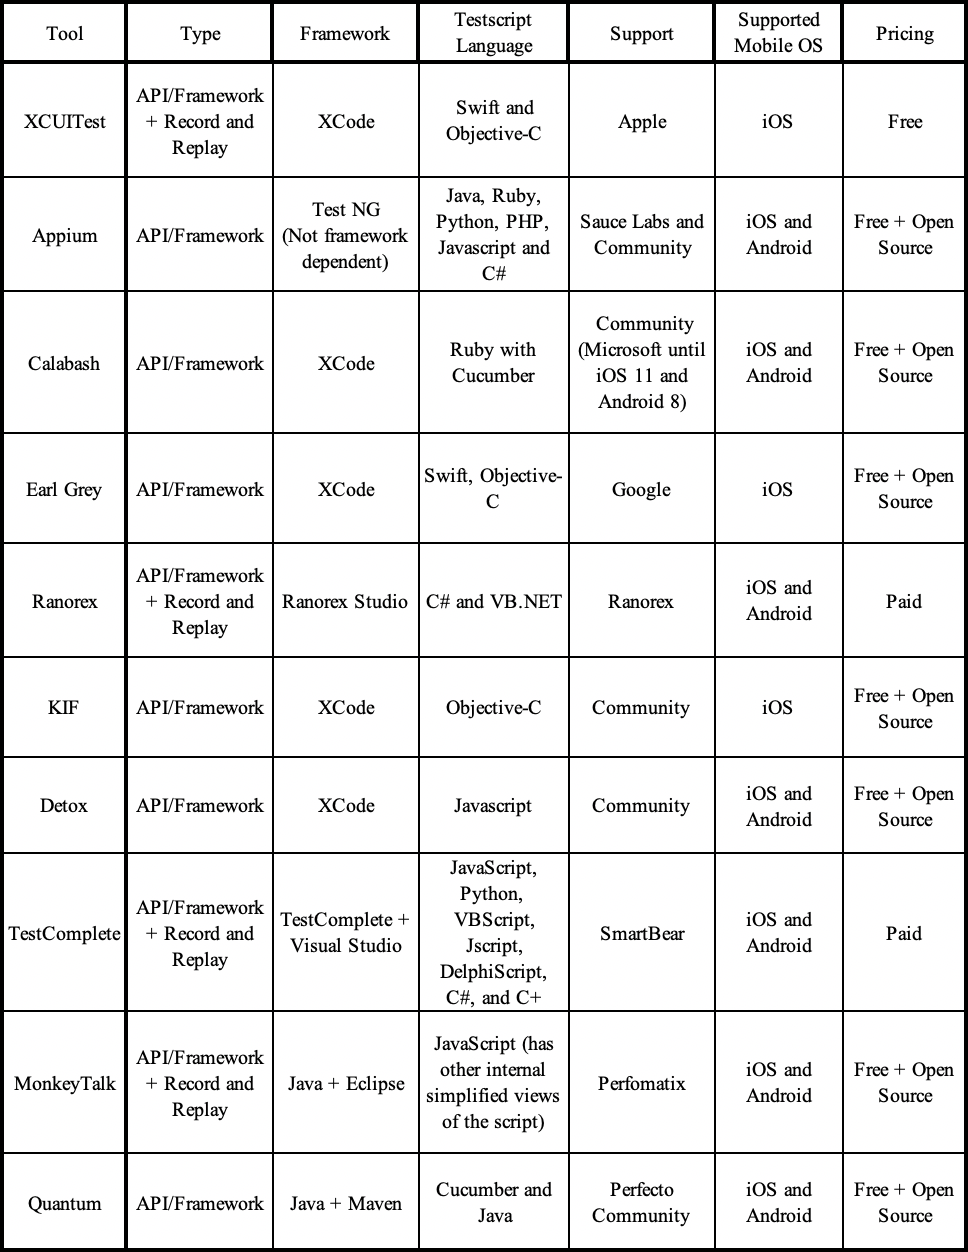
\includegraphics[width=12cm]{img/table1.png} \\[0mm]

\section{Categories}
In order to compare these test automation tools, it is important to understand the different elements, interactions and functionality a mobile application utilizes. These will be broken down in three categories: GUI components, Gestures and Testing Capabilities. The first makes reference to the all the elements that make up the graphical user interface, which can be divided into three categories: Bars, Views and Controls. Gestures are the main way users provide input to their mobile devices. Finally, testing capabilities make reference to the various APIs the test automation tool could provide in order to manipulate GUI elements, operating system and hardware configurations.

The following is a list of GUI components and gestures \cite{AppleHumanInterface}, as well as some of the testing capabilities that one may need while automating tests.

\subsection {GUI Components}
	
	Bars
	\begin{itemize}
  		\vspace{-0.4cm}\item Navigation Bar
  		\vspace{-0.4cm}\item Search Bars
		\vspace{-0.4cm}\item Status Bars
		\vspace{-0.4cm}\item Tab Bars
		\vspace{-0.4cm}\item Toolbars
	\end{itemize}

	Views
	\begin{itemize}
  		\vspace{-0.4cm}\item Action Sheets
		\vspace{-0.4cm}\item Activity Views
		\vspace{-0.4cm}\item Alerts
		\vspace{-0.4cm}\item Collections
		\vspace{-0.4cm}\item Image Views
		\vspace{-0.4cm}\item Pages
		\vspace{-0.4cm}\item Popovers
		\vspace{-0.4cm}\item Scroll Views
		\vspace{-0.4cm}\item Split Views
		\vspace{-0.4cm}\item Tables
		\vspace{-0.4cm}\item Text Views
		\vspace{-0.4cm}\item Web Views
	\end{itemize}
	
	Controls
	\begin{itemize}
  		\vspace{-0.4cm}\item Buttons
		\vspace{-0.4cm}\item Context Menus
		\vspace{-0.4cm}\item Edit Menus
		\vspace{-0.4cm}\item Labels
		\vspace{-0.4cm}\item Page Controls
		\vspace{-0.4cm}\item Pickers
		\vspace{-0.4cm}\item Progress Indicators
		\vspace{-0.4cm}\item Refresh Content Controls
		\vspace{-0.4cm}\item Segmented Controls
		\vspace{-0.4cm}\item Sliders
		\vspace{-0.4cm}\item Steppers
		\vspace{-0.4cm}\item Switches
		\vspace{-0.4cm}\item Text Fields
	\end{itemize}

\subsection {Gestures}

	\begin{itemize}
  		\vspace{-0.4cm}\item 3D Touch
		\vspace{-0.4cm}\item Tap
		\vspace{-0.4cm}\item Drag
		\vspace{-0.4cm}\item Flick
		\vspace{-0.4cm}\item Swipe
		\vspace{-0.4cm}\item Double tap
		\vspace{-0.4cm}\item Pinch
		\vspace{-0.4cm}\item Touch and Hold
		\vspace{-0.4cm}\item Shake
		\vspace{-0.4cm}\item Rotate
	\end{itemize}

\subsection {Framework Testing Capabilities}
	\begin{itemize}
  		\vspace{-0.4cm}\item Element handling: Element searching and Element attributes
		\vspace{-0.4cm}\item Authentication: Touch ID and Face ID
		\vspace{-0.4cm}\item Toggle hardware configurations: Wi-Fi, Data, Bluetooth, …
		\vspace{-0.4cm}\item Access system configurations: Language, Region, Time, Text Size, …
		\vspace{-0.4cm}\item Change device orientation
		\vspace{-0.4cm}\item GPS mocking
		\vspace{-0.4cm}\item Camera mocking
		\vspace{-0.4cm}\item Application state (set app to background, reopen app)
		\vspace{-0.4cm}\item Multitasking
		\vspace{-0.4cm}\item Notification handling
		\vspace{-0.4cm}\item Access app cache  data
		\vspace{-0.4cm}\item File handling
	\end{itemize}
	
\subsection {Automation Tool Characteristics and Features}

Other important aspects to take into account when evaluating the suitability of a test automation tool for a project are the characteristics and features provided by the framework. Some of these may become invaluable depending on the project. 

Examples for such are: 
	\begin{itemize}
  		\vspace{-0.4cm}\item Performance: Test execution time, memory use, …
		\vspace{-0.4cm}\item Maintainability
		\vspace{-0.4cm}\item Test parallelization
		\vspace{-0.4cm}\item Emulated and Real Device compatibility
		\vspace{-0.4cm}\item Ease of development (skill required)
		\vspace{-0.4cm}\item Android (hybrid) project compatibility
		\vspace{-0.4cm}\item Programming Languages Supported
		\vspace{-0.4cm}\item Developer Support
		\vspace{-0.4cm}\item Price
	\end{itemize}

